\documentclass[tikz,border=8pt]{standalone}
% Shared look for every TikZ diagram. Load with % Shared look for every TikZ diagram. Load with % Shared look for every TikZ diagram. Load with \input{../../tools/tikz-style.tex}
\usepackage[T1]{fontenc}
\usepackage{lmodern}
\renewcommand{\sfdefault}{lmr}  % diagrams use the same serif as the text
\usetikzlibrary{arrows.meta, positioning, shapes.geometric, calc, fit, backgrounds}
\definecolor{cblue}{HTML}{4C78A8}
\definecolor{corange}{HTML}{F58518}
\definecolor{cgreen}{HTML}{54A24B}
\definecolor{cred}{HTML}{E45756}
\definecolor{cpurple}{HTML}{B279A2}
\definecolor{cgrey}{HTML}{6B6B6B}
\tikzset{
  every picture/.style={font=\sffamily, line width=1.2pt},
  box/.style={draw=#1, fill=#1!12, rounded corners=4pt, align=center, inner sep=7pt, minimum height=1.1cm},
  box/.default=cgrey,
  arrow/.style={-{Stealth[length=3mm]}, draw=cgrey, line width=1.4pt},
  title/.style={font=\sffamily\bfseries\Large},
  note/.style={font=\sffamily\small, text=cgrey, align=center},
}
\AtBeginDocument{\hyphenpenalty=10000 \exhyphenpenalty=10000}

\usepackage[T1]{fontenc}
\usepackage{lmodern}
\renewcommand{\sfdefault}{lmr}  % diagrams use the same serif as the text
\usetikzlibrary{arrows.meta, positioning, shapes.geometric, calc, fit, backgrounds}
\definecolor{cblue}{HTML}{4C78A8}
\definecolor{corange}{HTML}{F58518}
\definecolor{cgreen}{HTML}{54A24B}
\definecolor{cred}{HTML}{E45756}
\definecolor{cpurple}{HTML}{B279A2}
\definecolor{cgrey}{HTML}{6B6B6B}
\tikzset{
  every picture/.style={font=\sffamily, line width=1.2pt},
  box/.style={draw=#1, fill=#1!12, rounded corners=4pt, align=center, inner sep=7pt, minimum height=1.1cm},
  box/.default=cgrey,
  arrow/.style={-{Stealth[length=3mm]}, draw=cgrey, line width=1.4pt},
  title/.style={font=\sffamily\bfseries\Large},
  note/.style={font=\sffamily\small, text=cgrey, align=center},
}
\AtBeginDocument{\hyphenpenalty=10000 \exhyphenpenalty=10000}

\usepackage[T1]{fontenc}
\usepackage{lmodern}
\renewcommand{\sfdefault}{lmr}  % diagrams use the same serif as the text
\usetikzlibrary{arrows.meta, positioning, shapes.geometric, calc, fit, backgrounds}
\definecolor{cblue}{HTML}{4C78A8}
\definecolor{corange}{HTML}{F58518}
\definecolor{cgreen}{HTML}{54A24B}
\definecolor{cred}{HTML}{E45756}
\definecolor{cpurple}{HTML}{B279A2}
\definecolor{cgrey}{HTML}{6B6B6B}
\tikzset{
  every picture/.style={font=\sffamily, line width=1.2pt},
  box/.style={draw=#1, fill=#1!12, rounded corners=4pt, align=center, inner sep=7pt, minimum height=1.1cm},
  box/.default=cgrey,
  arrow/.style={-{Stealth[length=3mm]}, draw=cgrey, line width=1.4pt},
  title/.style={font=\sffamily\bfseries\Large},
  note/.style={font=\sffamily\small, text=cgrey, align=center},
}
\AtBeginDocument{\hyphenpenalty=10000 \exhyphenpenalty=10000}

\begin{document}
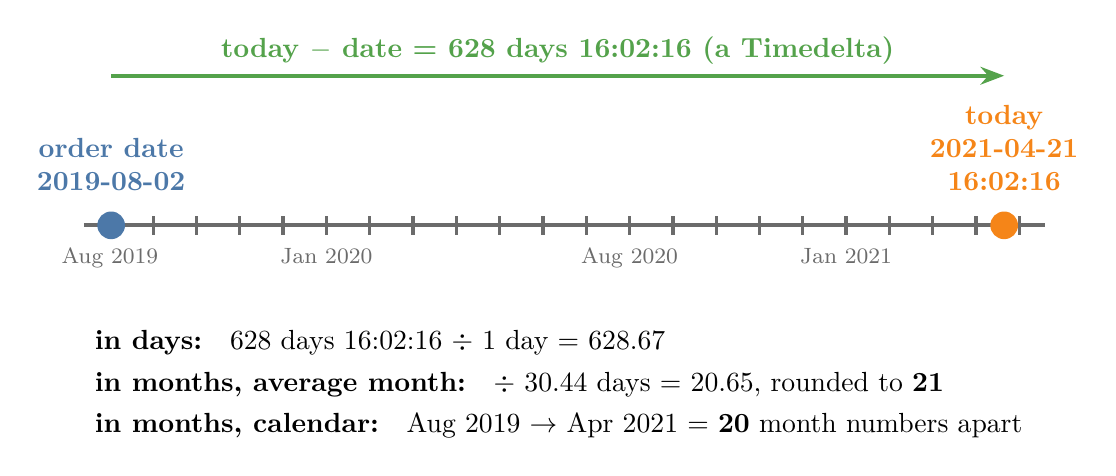
\begin{tikzpicture}[x=0.55cm]
  % timeline: x = months after 2019-08-01 (day offsets scaled to 1/30)
  \def\start{0.03}   % 2 Aug 2019
  \def\stop{20.65}   % 21 Apr 2021, afternoon
  \draw[line width=1.4pt, cgrey] (-0.6,0) -- (21.6,0);
  \foreach \m in {0,...,21} \draw[cgrey] (\m,-0.12) -- (\m,0.12);
  \foreach \m/\l in {0/Aug 2019, 5/Jan 2020, 12/Aug 2020, 17/Jan 2021}
    \node[note, below, font=\sffamily\footnotesize] at (\m,-0.15) {\l};
  % the two dates
  \fill[cblue] (\start,0) circle (5pt);
  \node[font=\sffamily\bfseries, text=cblue, above=0.3cm, align=center] at (\start,0) {order date\\2019-08-02};
  \fill[corange] (\stop,0) circle (5pt);
  \node[font=\sffamily\bfseries, text=corange, above=0.3cm, align=center] at (\stop,0) {today\\2021-04-21\\16:02:16};
  % the Timedelta
  \draw[arrow, cgreen] (\start,1.9) -- node[above, font=\sffamily\bfseries, text=cgreen] {today $-$ date = 628 days 16:02:16 (a Timedelta)} (\stop,1.9);
  % ways to turn it into a number
  \node[anchor=north west, align=left, font=\sffamily] at (-0.6,-1.2) {%
    \textbf{in days:}\quad 628 days 16:02:16 $\div$ 1 day $=$ 628.67\\[3pt]
    \textbf{in months, average month:}\quad $\div$ 30.44 days $=$ 20.65, rounded to \textbf{21}\\[3pt]
    \textbf{in months, calendar:}\quad Aug 2019 $\rightarrow$ Apr 2021 $=$ \textbf{20} month numbers apart};
\end{tikzpicture}
\end{document}
